% Compile: latexmk -xelatex time_to_acceleration_case_a_zh.tex
\documentclass[UTF8,fontset=fandol,11pt,a4paper]{ctexart}
\usepackage[margin=22mm,headheight=15pt]{geometry}
\usepackage{amsmath,amssymb,booktabs,array,xcolor,tikz,fancyhdr,hyperref}
\usepackage{enumitem}
\setlist{topsep=3pt,itemsep=2pt,parsep=0pt}
\usetikzlibrary{arrows.meta,positioning}
\definecolor{Navy}{HTML}{17334D}
\definecolor{Teal}{HTML}{007E87}
\definecolor{Amber}{HTML}{AF6D14}
\hypersetup{colorlinks=true,linkcolor=Teal,urlcolor=Teal,pdftitle={从冲突时间到加减速度：Case A 与 Case B 推演}}
\pagestyle{fancy}\fancyhf{}
\fancyhead[L]{\small\textcolor{Navy}{Decision--Barrier Framework}}
\fancyhead[R]{\small 时间约束与加速度协调}
\fancyfoot[C]{\small\thepage}
\setlength{\parindent}{0pt}
\setlength{\parskip}{6pt}
\renewcommand{\arraystretch}{1.25}
\ctexset{section={format=\Large\bfseries\color{Navy}},subsection={format=\normalsize\bfseries\color{Teal}}}
\newcommand{\nom}{\mathrm{nom}}
\newcommand{\dd}{\mathrm{d}}
\newcommand{\unit}[1]{\,\mathrm{#1}}
\newcommand{\key}[1]{\begin{quote}\color{Teal}\bfseries #1\end{quote}}
\begin{document}
\begin{center}
{\LARGE\bfseries\color{Navy}从冲突时间到加减速度}\par\vspace{5pt}
{\large 有序时间裕量、联合优化与 Case A / Case B 数值推演}\par\vspace{5pt}
{\small 方法说明笔记\quad |\quad 2026 年 9 月 24 日}
\end{center}

\section{先明确：约束决定能做什么，目标决定选哪个值}
对于交叉车流，单独计算每对车辆的制动修正，再把修正相加，并不能保证最后的加速度满足每一组冲突要求。同一辆车只有一个纵向加速度，却可能同时面对多个冲突点。

\key{正确的接口是：决策层确定先后关系；安全层把每个时间要求写成加速度约束；联合优化在所有约束的交集中选择控制。}

\begin{center}
\begin{tikzpicture}[node distance=5mm,>=Latex,
  box/.style={draw=Teal,rounded corners,fill=Teal!4,text width=12.7cm,align=center,minimum height=9mm,font=\small}]
\node[box](a){测量距离、速度与路径；确认本周期有效的通行顺序};
\node[box,below=of a](b){由期望速度与跟车状态计算名义加速度 $u_i^{\nom}$};
\node[box,below=of b](c){计算 $T_i^m$、有序时间裕量 $h_{ij}^m$，更新全部加速度约束};
\node[box,below=of c](d){联合求解 $\mathbf u^*$，执行一个控制周期，然后反馈更新};
\draw[->](a)--(b);\draw[->](b)--(c);\draw[->](c)--(d);
\end{tikzpicture}
\end{center}

\subsection{变量与本笔记的工作范围}
\begin{center}\small
\begin{tabular}{p{3.1cm}p{10.5cm}}
\toprule
符号 & 含义与单位\\\midrule
$d_i^m$ & 车辆 $i$ 沿既定路径到冲突点 $c_m$ 的剩余距离，m\\
$v_i,\ u_i$ & 速度（m/s）、纵向加速度（m/s$^2$），负加速度表示制动\\
$T_i^m=d_i^m/v_i$ & 按当前速度外推的剩余到达时间，s；不是已预约的时刻\\
$\tau_m,\ h_{ij}^m$ & 要求的时间间隔与剩余时间裕量，s\\
$\kappa_m$ & 裕量约束参数，s$^{-1}$\\\bottomrule
\end{tabular}\end{center}

以下推导限定于固定路径、固定顺序、接近阶段和正速度工作区间 $v_i>v_{\mathrm{switch}}>0$，并将 $\tau_m$ 设为常数。先假设协调器能获得各车状态并联合下发加速度。

这是对当前 Idea Note 的控制接口补充。数值例子用于演示计算过程，不代表已完成实体车辆碰撞安全证明或完整路口仿真。

\newpage
\section{从到达时间推导加速度约束}
\subsection{第一步：用顺序定义有方向的裕量}
若车辆 $i$ 先于车辆 $j$ 通过冲突点 $c_m$，定义
\begin{equation}
h_{ij}^m=T_j^m-T_i^m-\tau_m\geq0.
\end{equation}
它同时表达“$i$ 先、$j$ 后”与“预计到达时间至少相隔 $\tau_m$”。绝对值形式只表达间隔，不能单独指定顺序。

\subsection{第二步：对时间裕量求导}
车辆模型与到达时间估计为
\begin{equation}
\dot d_i^m=-v_i,\qquad \dot v_i=u_i,\qquad T_i^m=\frac{d_i^m}{v_i}.
\end{equation}
按商的求导法则，
\begin{equation}
\dot T_i^m=\frac{\dot d_i^m v_i-d_i^m\dot v_i}{v_i^2}
=-1-\frac{d_i^m}{v_i^2}u_i.
\end{equation}
匀速时剩余时间每秒减少一秒；加速使它下降得更快，减速则使它下降得更慢。因此
\begin{equation}
\dot h_{ij}^m=\frac{d_i^m}{v_i^2}u_i-\frac{d_j^m}{v_j^2}u_j.
\end{equation}

\subsection{第三步：限制裕量下降速度}
采用候选控制屏障条件 $\dot h_{ij}^m+\kappa_m h_{ij}^m\geq0$，得到
\begin{equation}\boxed{
\frac{d_i^m}{v_i^2}u_i-\frac{d_j^m}{v_j^2}u_j
+\kappa_m h_{ij}^m\geq0.}
\label{eq:cbf}
\end{equation}
每次更新时，距离与速度都是已知量，式\eqref{eq:cbf}是关于加速度的线性约束。在 $h=0$ 时，它要求 $\dot h\geq0$；在 $h>0$ 时，允许裕量适度下降。若该微分不等式在模型有效期间持续成立，则 $h(t)\geq h(0)e^{-\kappa t}$。这需要初始裕量非负与控制持续可行等条件。

\subsection{第四步：在允许的加速度中选取最接近名义控制的值}
\begin{equation}
\begin{aligned}
\min_{\mathbf u}\quad &\frac12\sum_i q_i(u_i-u_i^{\nom})^2,\qquad q_i>0,\\
\text{s.t.}\quad &\dot h_{ij}^m+\kappa_mh_{ij}^m\geq0\quad\text{（所有相关冲突对）},\\
&u_{i,\min}\leq u_i\leq u_{i,\max},\quad\text{以及适用的速度、跟车约束。}
\end{aligned}
\end{equation}
这个二次规划（QP）同时选择各车加速度。求解后可定义 $u_i^{\mathrm{barrier}}=u_i^*-u_i^{\nom}$，保留“名义控制加安全修正”的结构，无需将各冲突的修正单独相加。

\newpage
\section{Case A：三条有向车道、两组交叉冲突}
南北道路双向，东西道路仅允许从东向西行驶。每条车道选一辆接近车辆：A 位于 $l_{EW}$，B 位于 $l_{SN}$，C 位于 $l_{NS}$。本例按 A 的行驶先后编号：先遇 $c_1$，再遇 $c_2$。

\begin{center}
\begin{tikzpicture}[x=1cm,y=1cm,>=Latex]
\fill[gray!10](-1.5,-2.1)rectangle(1.5,2.1);
\fill[gray!10](-5,-.5)rectangle(5,.5);
\draw[dashed,white,line width=1.5pt](0,-2.1)--(0,2.1);
\draw[->,very thick,Amber](4.7,0)--(-4.7,0);
\draw[->,very thick,Teal](.75,-1.9)--(.75,1.9);
\draw[->,very thick,Navy](-.75,1.9)--(-.75,-1.9);
\node[fill=Amber,text=white,rounded corners,minimum width=9mm]at(3.3,0){A};
\node[fill=Teal,text=white,rounded corners]at(.75,-1.45){B};
\node[fill=Navy,text=white,rounded corners]at(-.75,1.45){C};
\filldraw[fill=white,draw=black](.75,0)circle(.08);
\filldraw[fill=white,draw=black](-.75,0)circle(.08);
\node[above right]at(.85,.1){$c_1$};\node[above left]at(-.85,.1){$c_2$};
\node[above,text=Amber]at(3.5,.5){$l_{EW}$：东 $\to$ 西};
\node[right,text=Teal]at(1,-1.5){$l_{SN}$：南 $\to$ 北};
\node[left,text=Navy]at(-1,1.5){$l_{NS}$：北 $\to$ 南};
\draw[<->](-.75,-.85)--(.75,-.85);
\node[below,fill=white,inner sep=1pt]at(0,-.85){$4\unit{m}$};
\end{tikzpicture}

{\small 图为拓扑示意，车辆位置不按数值距离比例绘制。}
\end{center}

两组交叉冲突为 $(A,B)$ 在 $c_1$ 相交、$(A,C)$ 在 $c_2$ 相交。B 与 C 位于不同的对向车道，直行路径在本例中不相交。

\subsection{初始状态与决策顺序}
\begin{center}
\begin{tabular}{ccrrl}
\toprule
车辆 & 冲突点 & 距离（m） & 速度（m/s） & $T$（s）\\\midrule
A & $c_1$ & 50 & 10 & 5.0\\
A & $c_2$ & 54 & 10 & 5.4\\
B & $c_1$ & 28 & 10 & 2.8\\
C & $c_2$ & 76 & 10 & 7.6\\\bottomrule
\end{tabular}
\end{center}
两冲突点沿 A 路径相距 4 m，故始终有 $d_A^2=d_A^1+4$。采用共同优先关系 $B\prec A\prec C$，在各冲突点分别导出 $B\prec A$ 和 $A\prec C$；不对不存在冲突的 B、C 另加交叉约束。

取 $\tau_1=\tau_2=2\unit{s}$、$\kappa_1=\kappa_2=1\unit{s^{-1}}$，则
\[
h_1=T_A^1-T_B^1-2=0.2\unit{s},\qquad
h_2=T_C^2-T_A^2-2=0.2\unit{s}.
\]
两组初始时间裕量均为正。本例的 2 秒是用于推演的设定值，尚未根据车身长度与区域清空时间标定。

\newpage
\section{把 Case A 完整算一遍：从参考值到最优加速度}
\subsection{名义控制提供参考值}
本例每条车道只有一辆车，无同车道前车，采用巡航参考
\[
u_i^{\nom}=k_v(v_i^{\mathrm{des}}-v_i),\qquad k_v=0.5\unit{s^{-1}}.
\]
设 $(v_A^{\mathrm{des}},v_B^{\mathrm{des}},v_C^{\mathrm{des}})=(12,10,12)\unit{m/s}$，得到
\[
\mathbf u^{\nom}=(1,0,1)^{\mathsf T}\unit{m/s^2}.
\]
\subsection{两组时间要求变为两个共同约束}
在 $c_1$，B 先 A 后；在 $c_2$，A 先 C 后。由式\eqref{eq:cbf}，
\begin{align}
-0.50u_A+0.28u_B+0.20&\geq0,\label{eq:first}\\
0.54u_A-0.76u_C+0.20&\geq0.\label{eq:second}
\end{align}
代入名义控制，左侧分别为 $-0.30$ 与 $-0.02$，均不满足。因此要调整控制，不能直接执行 $(1,0,1)$。

取相等权重，以及 $-3\leq u_i\leq2\unit{m/s^2}$，求解
\[
\min\ \frac12\big[(u_A-1)^2+u_B^2+(u_C-1)^2\big]
\quad\text{满足式\eqref{eq:first}、\eqref{eq:second}和加速度边界。}
\]
\subsection{手算候选解，并检查最优性}
对本组数值，两条冲突约束在最优点均取等号。先按该活跃集合求候选值：
\[
u_B=\frac{0.50u_A-0.20}{0.28},\qquad
u_C=\frac{0.54u_A+0.20}{0.76}.
\]
令 $x=u_A$，代入目标并求导：
\[
0=(x-1)+\frac{0.50(0.50x-0.20)}{0.28^2}
+\frac{0.54(0.54x-0.56)}{0.76^2}.
\]
解得
\begin{equation}\boxed{
(u_A^*,u_B^*,u_C^*)=(0.596353,\ 0.350630,\ 0.686882)\unit{m/s^2}.}
\end{equation}
各输入均在边界内。两约束的非负 KKT 乘子约为 $(1.252251,0.411997)$，满足驻点与互补条件；由于目标严格凸，该可行候选即唯一最优解。一般情形不能预先假定全部约束取等号，应由求解器判断。

\key{A 少加速以让 B 先行；B 适当加速帮助清空第一个冲突；C 少加速以让 A 先行。这次不需要刹车，而是三车共同调整加速强度。}

\newpage
\section{0.1 秒后：距离、速度与加速度一起更新}
采用采样周期 $\Delta t=0.1\unit{s}$，在一个周期内保持求得的加速度不变。理想双积分模型给出精确的周期更新：
\begin{align}
v_i^{+}&=v_i+u_i^*\Delta t,\\
(d_i^m)^{+}&=d_i^m-v_i\Delta t-\tfrac12u_i^*\Delta t^2.
\end{align}
代入初始解，得到 $t=0.1\unit{s}$ 时的状态：
\begin{center}\small
\begin{tabular}{ccrrr}
\toprule
车辆 & 冲突点 & 新距离（m） & 新速度（m/s） & 新 $T$（s）\\\midrule
A & $c_1$ & 48.997018 & 10.059635 & 4.870656\\
A & $c_2$ & 52.997018 & 10.059635 & 5.268284\\
B & $c_1$ & 26.998247 & 10.035063 & 2.690391\\
C & $c_2$ & 74.996566 & 10.068688 & 7.448494\\\bottomrule
\end{tabular}\end{center}
因此
\[
h_1^+=0.180264\unit{s},\qquad h_2^+=0.180210\unit{s}.
\]
\textbf{裕量变小并不等于控制失效。}采用的约束允许正裕量下降，目标是在尽量保留名义控制的同时不越过边界，而不是让 $h$ 一直增大。

此时名义加速度也重算为
\[
(u_A^{\nom},u_B^{\nom},u_C^{\nom})
\approx(0.970182,-0.017532,0.965656)\unit{m/s^2}.
\]
用新距离、速度更新两个约束的所有系数，重新求解得到
\[
\boxed{\mathbf u^+(0.1)\approx(0.559344,\ 0.337778,\ 0.639581)^{\mathsf T}\unit{m/s^2}.}
\]
\subsection{连续十个控制周期的局部演算}
\begin{center}\small
\begin{tabular}{rrrrrr}
\toprule
$t$（s） & $h_1$（s） & $h_2$（s） & $u_A$ & $u_B$ & $u_C$\\\midrule
0.0 & 0.200000 & 0.200000 & 0.596353 & 0.350630 & 0.686882\\
0.1 & 0.180264 & 0.180210 & 0.559344 & 0.337778 & 0.639581\\
0.2 & 0.162466 & 0.162365 & 0.524012 & 0.324840 & 0.594765\\
0.5 & 0.118895 & 0.118696 & 0.427264 & 0.285069 & 0.474350\\
1.0 & 0.070581 & 0.070327 & 0.292552 & 0.213336 & 0.314795\\\bottomrule
\end{tabular}\end{center}
加速度单位均为 m/s$^2$，每行表示该时刻新求得的指令。计算使用未舍入数值，表中仅显示六位小数。1 ms 间隔的周期内数值回放得到最小时间裕量约 $0.070327\unit{s}$；这只是本段 1 秒轨迹的检查，不是采样间安全证明，也没有演示车辆完成过路口。

\newpage
\section{如何落地，以及哪些结论尚不能宣称}
\subsection{每个控制周期的执行顺序}
\begin{enumerate}
\item 获取各车状态与路径，保留有效的冲突对及已承诺的通行顺序。
\item 计算名义加速度，更新每个冲突点的剩余距离、到达估计与时间裕量。
\item 将所有有序时间约束放入同一个 QP，并加入车辆输入、速度与跟车约束。
\item 检查是否有可行解；有解则执行本周期指令，并记录实际响应。
\item 下一周期重新测量并求解。指令实时更新，通行顺序不因轻微速度变化频繁翻转。
\end{enumerate}

\subsection{这份推导解决了什么}
它将原来的“每个冲突给一个修正，再求和”改为“每个冲突给一个约束，再联合求解”。名义控制提供加速度参考，目标函数选择共同可行值。Case A 展示了同一辆 A 的输入如何同时受到两个冲突点约束。

\subsection{继续扩展时必须处理的边界}
\begin{itemize}
\item \textbf{低速与停车：} $d/v$ 的推导不能直接用于 $v=0$；将分母换成 $\max(v,v_{\min})$ 后也不能照搬导数。需要停止、等待、放行模式及切换条件。
\item \textbf{车身占用：} 到达参考点的时间间隔不是完整的区域占用安全条件。应检查先行车辆清空区域与后行车辆进入区域的关系，考虑车长、车速和冲突区域几何。
\item \textbf{采样与误差：} 连续时间条件在采样点成立，不自动保证整个保持区间都成立。后续需考虑采样裕量、感知误差、执行延迟或离散时间设计。
\item \textbf{初始状态与改序：} 新顺序需要检查对应的 $h\geq0$ 与输入可行性；当前已经 $h<0$ 时，不能借用“保持安全集合”的结论。承诺后也不能靠任意改序解决矛盾。
\item \textbf{QP 无解：} 说明当前约束没有共同可行输入。需在仍有制动余量时调整协调方案或进入经验证的应急机制；不能简单截断输出或放松硬安全约束后继续宣称安全。
\end{itemize}

\subsection{附件与复现}
本笔记依据当前项目的 Idea Note 与讨论进行代数推演。配套文件位于同一目录：
\begin{itemize}
\item \texttt{time\_to\_acceleration\_case\_a\_zh.tex}：本文可编辑 LaTeX 源码；
\item \texttt{time\_to\_acceleration\_case\_a.py}：仅用 Python 标准库，枚举活跃集并核验 KKT 条件；
\item \texttt{time\_to\_acceleration\_case\_a.csv}：每个采样点的距离、速度、参考控制、裕量与求解结果。
\end{itemize}
在本目录运行 \texttt{python3 time\_to\_acceleration\_case\_a.py} 可复算数值；运行 \texttt{latexmk -xelatex time\_to\_acceleration\_case\_a\_zh.tex} 可编译本文。代码采用理想共享状态与加速度执行，仅验证这个局部算例。
\newpage
\section{Case B：四条有向车道与冲突矩阵}
在 Case A 的基础上增加西向东车道及车辆 D，两条道路均变为双向。仍只考虑直行，每条有向车道一辆车。A、B、C 的原车道与 $c_1,c_2$ 编号保持不变，新增 $c_3,c_4$。
\begin{center}
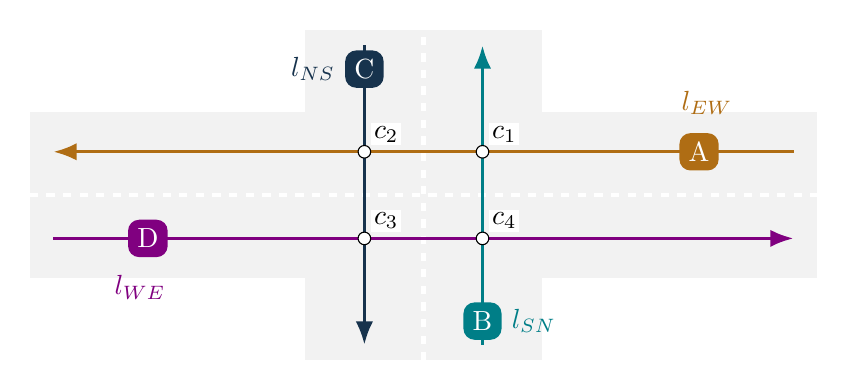
\begin{tikzpicture}[x=1cm,y=1cm,>=Latex]
\fill[gray!10](-1.5,-2.1)rectangle(1.5,2.1);
\fill[gray!10](-5,-1.05)rectangle(5,1.05);
\draw[dashed,white,line width=1.5pt](0,-2.1)--(0,2.1);
\draw[dashed,white,line width=1.5pt](-5,0)--(5,0);
\draw[->,very thick,Amber](4.7,.55)--(-4.7,.55);
\draw[->,very thick,violet](-4.7,-.55)--(4.7,-.55);
\draw[->,very thick,Teal](.75,-1.9)--(.75,1.9);
\draw[->,very thick,Navy](-.75,1.9)--(-.75,-1.9);
\node[fill=Amber,text=white,rounded corners]at(3.5,.55){A};
\node[fill=violet,text=white,rounded corners]at(-3.5,-.55){D};
\node[fill=Teal,text=white,rounded corners]at(.75,-1.6){B};
\node[fill=Navy,text=white,rounded corners]at(-.75,1.6){C};
\foreach \x/\y/\n in {.75/.55/1,-.75/.55/2,-.75/-.55/3,.75/-.55/4}{
\filldraw[fill=white,draw=black](\x,\y)circle(.08);
\node[above right,fill=white,inner sep=1pt]at(\x+.08,\y+.08){$c_{\n}$};}
\node[above,text=Amber]at(3.6,.9){$l_{EW}$};
\node[below,text=violet]at(-3.6,-.9){$l_{WE}$};
\node[right,text=Teal]at(1,-1.6){$l_{SN}$};
\node[left,text=Navy]at(-1,1.6){$l_{NS}$};
\end{tikzpicture}

{\small 拓扑示意，不按距离比例绘制；沿每条路径的两冲突点间距均取 4 m。}
\end{center}
\subsection{矩阵记录谁与谁存在几何冲突}
固定行列顺序为车辆 $(A,B,C,D)$，对应车道 $(l_{EW},l_{SN},l_{NS},l_{WE})$，冲突矩阵为
\begin{equation}
G=\begin{bmatrix}
0&1&1&0\\1&0&0&1\\1&0&0&1\\0&1&1&0
\end{bmatrix}.
\end{equation}
$G_{ij}=1$ 表示直行路径相交；对角线为零。只遍历上三角非零元，得到四个唯一冲突对 $(A,B)$、$(A,C)$、$(B,D)$、$(C,D)$，不能把对称元素重复计数。

若按照原稿的分组顺序 $(B,C,A,D)$ 排列，即先南北两车道、再东西两车道，同一关系写为
\[
G'=\begin{bmatrix}0&0&1&1\\0&0&1&1\\1&1&0&0\\1&1&0&0\end{bmatrix}.
\]
两者仅行列排列不同。以下控制向量始终采用 $\mathbf u=(u_A,u_B,u_C,u_D)^{\mathsf T}$。
\key{冲突矩阵描述“谁需要协调”，不决定“谁先走”。先后关系由决策层给出，几何冲突、通行顺序和实时状态共同生成控制约束。}
\textbf{本例范围：} B 与 C、A 与 D 分别沿分离的对向车道直行，因此不构成交叉冲突；这不适用于任意转弯场景。相同车道后续车辆的追尾安全也不由这个矩阵负责。

\newpage
\section{Case B：从初始状态建立四条约束}
\subsection{保持路径距离一致，指定共同通行顺序}
四车初始速度均为 $10\unit{m/s}$。A 先经过 $c_1$ 再经过 $c_2$；B 先 $c_4$ 后 $c_1$；C 先 $c_2$ 后 $c_3$；D 先 $c_3$ 后 $c_4$。
\begin{center}\small
\begin{tabular}{clrr}
\toprule
车辆 & 沿路径的冲突点顺序 & 两处距离（m） & 两处 $T$（s）\\\midrule
A & $c_1\to c_2$ & $50,\ 54$ & $5.0,\ 5.4$\\
B & $c_4\to c_1$ & $24,\ 28$ & $2.4,\ 2.8$\\
C & $c_2\to c_3$ & $76,\ 80$ & $7.6,\ 8.0$\\
D & $c_3\to c_4$ & $102,\ 106$ & $10.2,\ 10.6$\\\bottomrule
\end{tabular}\end{center}
决策层采用一致优先关系 $B\prec A\prec C\prec D$，并仅在确实存在冲突的车辆对上导出约束。取 $\tau_m=2\unit{s}$、$\kappa_m=1\unit{s^{-1}}$。
\begin{center}\small
\begin{tabular}{cclc}
\toprule
冲突点 & 先后关系 & 时间裕量定义 & 初始裕量（s）\\\midrule
$c_1$ & $B\prec A$ & $h_1=T_A^1-T_B^1-2$ & 0.2\\
$c_2$ & $A\prec C$ & $h_2=T_C^2-T_A^2-2$ & 0.2\\
$c_3$ & $C\prec D$ & $h_3=T_D^3-T_C^3-2$ & 0.2\\
$c_4$ & $B\prec D$ & $h_4=T_D^4-T_B^4-2$ & 6.2\\\bottomrule
\end{tabular}\end{center}
这里的优先序不要求 B 完全离开整个路口后 A 才能进入，而是在每个共用冲突点上落实先后关系。尤其不能因为 B、D 不在全局队列中相邻，就漏掉 $c_4$ 的直接冲突检查。

\subsection{逐项代入控制屏障条件}
\begin{align}
c_1:\quad -0.50u_A+0.28u_B+0.20&\geq0,\\
c_2:\quad 0.54u_A-0.76u_C+0.20&\geq0,\\
c_3:\quad 0.80u_C-1.02u_D+0.20&\geq0,\\
c_4:\quad 0.24u_B-1.06u_D+6.20&\geq0.
\end{align}
写成矩阵形式为
\begin{equation}
\underbrace{\begin{bmatrix}
-.50&.28&0&0\\.54&0&-.76&0\\0&0&.80&-1.02\\0&.24&0&-1.06
\end{bmatrix}}_{M(0)}\mathbf u+
\underbrace{\begin{bmatrix}.20\\.20\\.20\\6.20\end{bmatrix}}_{\mathbf h(0)}\geq\mathbf0.
\end{equation}
$G$ 是几何邻接矩阵；$M(t)$ 是由距离、速度、顺序实时生成的控制约束矩阵。本例 $\kappa_m=1$，故右侧裕量项数值恰为 $\mathbf h$；一般应写为 $M(t)\mathbf u+\operatorname{diag}(\kappa_m)\mathbf h(t)\geq0$。

\newpage
\section{Case B：联合选取四辆车的加速度}
\subsection{先给参考控制，再判断哪些约束需要干预}
沿用 $u_i^{\nom}=0.5(v_i^{\mathrm{des}}-v_i)$，设期望速度为 $(12,10,12,12)\unit{m/s}$，得到 $\mathbf u^{\nom}=(1,0,1,1)^{\mathsf T}\unit{m/s^2}$。

代入四条约束，左侧分别为 $(-0.30,-0.02,-0.02,5.14)$。前三条不满足，第四条满足，但四条都进入联合问题：
\[
\begin{aligned}
\min_{\mathbf u}\quad &\tfrac12[(u_A-1)^2+u_B^2+(u_C-1)^2+(u_D-1)^2],\\
\text{s.t.}\quad &M(0)\mathbf u+\mathbf h(0)\geq\mathbf0,\qquad -3\leq u_i\leq2.
\end{aligned}
\]
\subsection{把活跃约束代回目标，演算候选解}
本组数值的最优点上，前三条约束取等号，第四条为非活跃约束。以 $x=u_A$，可写成
\[
b(x)=\frac{0.50x-0.20}{0.28},\qquad
c(x)=\frac{0.54x+0.20}{0.76},\qquad
d(x)=\frac{0.80c(x)+0.20}{1.02}.
\]
于是只需对以下一元二次函数求驻点：
\[
f(x)=\tfrac12\big[(x-1)^2+b(x)^2+(c(x)-1)^2+(d(x)-1)^2\big],
\]
\[
0=f'(x)=(x-1)+\frac{0.50}{0.28}b(x)
+\frac{0.54}{0.76}(c(x)-1)
+\frac{0.80\cdot0.54}{1.02\cdot0.76}(d(x)-1).
\]
解得
\begin{equation}\boxed{
\mathbf u^*(0)=(0.625885,\ 0.403366,\ 0.707866,\ 0.751267)^{\mathsf T}\unit{m/s^2}.}
\end{equation}
代回后，四条约束左侧约为 $(0,0,0,5.500465)$。前三条约束的 KKT 乘子分别约为 $1.440593$、$0.641077$ 和 $0.243856$，均为正；第四条乘子为零，输入边界均未触及。因此候选满足最优性条件。代码实际枚举并检查活跃集，不预先强制前三条取等号。

\subsection{为什么增加 D，会改变原来三辆车的控制？}
\begin{center}\small
\begin{tabular}{crrrr}
\toprule
算例 & $u_A$ & $u_B$ & $u_C$ & $u_D$\\\midrule
Case A & .596353 & .350630 & .686882 & ---\\
Case B & .625885 & .403366 & .707866 & .751267\\\bottomrule
\end{tabular}\end{center}
新增 D 需要在 $c_3$ 配合 C；C 的动作又受 $c_2$ 的 A 约束，A 的动作受 $c_1$ 的 B 约束。因此协调会沿冲突关系传递，而不是只给 D 单独补一个修正。第四条约束虽有裕量，仍在每次更新时检查，不能永久删除。

\newpage
\section{Case B：更新状态、约束矩阵与下一周期控制}
仍令 $\Delta t=0.1\unit{s}$，保持初始加速度一个周期，并按前文双积分公式更新。为简化表格，每车仅列沿路径的第一个冲突点距离 $d_{i,\mathrm{first}}$；第二个距离始终加 4 m。
\begin{center}\small
\begin{tabular}{ccrrr}
\toprule
车辆 & 首个冲突点 & $d_{i,\mathrm{first}}^+$（m） & $v_i^+$（m/s） & $u_i^{\nom,+}$（m/s$^2$）\\\midrule
A & $c_1$ &48.996871&10.062589& .968706\\
B & $c_4$ &22.997983&10.040337&-.020168\\
C & $c_2$ &74.996461&10.070787& .964607\\
D & $c_3$ &100.996244&10.075127& .962437\\\bottomrule
\end{tabular}\end{center}
例如 $T_A^{1,+}=48.996871/10.062589\approx4.869211$，而
$T_B^{1,+}=(22.997983+4)/10.040337\approx2.688952$，故 $h_1^+\approx0.180259\unit{s}$。注意 B 到 $c_1$ 的距离必须加上两冲突点间的 4 m。

更新后的四条约束为 $M^+\mathbf u+\mathbf h^+\geq0$，其中
\[
M^+\approx\begin{bmatrix}
-.483893&.267815&0&0\\
.523396&0&-.739459&0\\
0&0&.778898&-.994957\\
0&.228136&0&-1.034362
\end{bmatrix},\qquad
\mathbf h^+\approx\begin{bmatrix}.180259\\.180208\\.180195\\6.130773\end{bmatrix}.
\]
使用新的名义控制重新求解，得到
\[
\boxed{\mathbf u^*(0.1)\approx(.588626,\ .390466,\ .660339,\ .698052)^{\mathsf T}\unit{m/s^2}.}
\]
\subsection{重复更新的结果}
\begin{center}\small
\begin{tabular}{rrrrr}
\toprule
$t$（s） & $h_1$（s） & $h_2$（s） & $h_3$（s） & $h_4$（s）\\\midrule
0.0&.200000&.200000&.200000&6.200000\\
0.1&.180259&.180208&.180195&6.130773\\
0.5&.118867&.118686&.118640&5.913428\\
1.0&.070524&.070309&.070258&5.739344\\\bottomrule
\end{tabular}\quad
\begin{tabular}{rrrrr}
\toprule
$t$（s）&$u_A$&$u_B$&$u_C$&$u_D$\\\midrule
0.0&.625885&.403366&.707866&.751267\\
0.1&.588626&.390466&.660339&.698052\\
0.5&.453918&.335659&.492937&.512793\\
1.0&.312576&.256143&.328307&.335897\\\bottomrule
\end{tabular}
\end{center}
加速度单位为 m/s$^2$。表格采用未舍入数据计算；每 1 ms 数值回放得到最小裕量约为 $0.070258\unit{s}$。这仍是正速度下的 1 秒局部演算，不是完整通行或实体碰撞安全验证。

\textbf{复算：}运行 \texttt{python3 time\_to\_acceleration\_case\_b.py}，将生成同名 CSV。脚本复用 Case A 中推广到任意小维度的活跃集求解器，检查可行性与 KKT 条件。CSV 中 $h_1,\ldots,h_4$ 按冲突点编号，$u_A,\ldots,u_D$ 按车辆编号。
\end{document}
